\documentclass[journal,12pt,twocolumn]{IEEEtran}
\usepackage{setspace}
\usepackage{gensymb}
\singlespacing
\usepackage[cmex10]{amsmath}
\usepackage{amsthm}
\usepackage{mathrsfs}
\usepackage{txfonts}
\usepackage{stfloats}
\usepackage{bm}
\usepackage{cite}
\usepackage{cases}
\usepackage{subfig}
\usepackage{longtable}
\usepackage{multirow}
\usepackage{enumitem}
\usepackage{mathtools}
\usepackage{tikz}
\usepackage{circuitikz}
\usepackage{verbatim}
\usepackage[breaklinks=true]{hyperref}
\usepackage{tkz-euclide} % loads  TikZ and tkz-base
\usepackage{listings}
\usepackage{color}    
\usepackage{array}    
\usepackage{longtable}
\usepackage{calc}     
\usepackage{multirow} 
\usepackage{hhline}   
\usepackage{ifthen}   
\usepackage{lscape}     
\usepackage{chngcntr}
\DeclareMathOperator*{\Res}{Res}
\renewcommand\thesection{\arabic{section}}
\renewcommand\thesubsection{\thesection.\arabic{subsection}}
\renewcommand\thesubsubsection{\thesubsection.\arabic{subsubsection}}

\renewcommand\thesectiondis{\arabic{section}}
\renewcommand\thesubsectiondis{\thesectiondis.\arabic{subsection}}
\renewcommand\thesubsubsectiondis{\thesubsectiondis.\arabic{subsubsection}}
\renewcommand\thetable{\arabic{table}}
% correct bad hyphenation here
\hyphenation{op-tical net-works semi-conduc-tor}
\def\inputGnumericTable{}                                 %%

\lstset{
%language=C,
frame=single, 
breaklines=true,
columns=fullflexible
}
%\lstset{
%language=tex,
%frame=single, 
%breaklines=true
%}

\begin{document}
\newtheorem{theorem}{Theorem}[section]
\newtheorem{problem}{Problem}
\newtheorem{proposition}{Proposition}[section]
\newtheorem{lemma}{Lemma}[section]
\newtheorem{corollary}[theorem]{Corollary}
\newtheorem{example}{Example}[section]
\newtheorem{definition}[problem]{Definition}
\newcommand{\BEQA}{\begin{eqnarray}}
\newcommand{\EEQA}{\end{eqnarray}}
\newcommand{\define}{\stackrel{\triangle}{=}}
\bibliographystyle{IEEEtran}
\providecommand{\mbf}{\mathbf}
\providecommand{\pr}[1]{\ensuremath{\Pr\left(#1\right)}}
\providecommand{\qfunc}[1]{\ensuremath{Q\left(#1\right)}}
\providecommand{\sbrak}[1]{\ensuremath{{}\left[#1\right]}}
\providecommand{\lsbrak}[1]{\ensuremath{{}\left[#1\right.}}
\providecommand{\rsbrak}[1]{\ensuremath{{}\left.#1\right]}}
\providecommand{\brak}[1]{\ensuremath{\left(#1\right)}}
\providecommand{\lbrak}[1]{\ensuremath{\left(#1\right.}}
\providecommand{\rbrak}[1]{\ensuremath{\left.#1\right)}}
\providecommand{\cbrak}[1]{\ensuremath{\left\{#1\right\}}}
\providecommand{\lcbrak}[1]{\ensuremath{\left\{#1\right.}}
\providecommand{\rcbrak}[1]{\ensuremath{\left.#1\right\}}}
\theoremstyle{remark}
\newtheorem{rem}{Remark}
\newcommand{\sgn}{\mathop{\mathrm{sgn}}}
\providecommand{\abs}[1]{\left\vert#1\right\vert}
\providecommand{\res}[1]{\Res\displaylimits_{#1}} 
\providecommand{\norm}[1]{\left\lVert#1\right\rVert}
\providecommand{\mtx}[1]{\mathbf{#1}}
\providecommand{\mean}[1]{E\left[ #1 \right]}
\providecommand{\fourier}{\overset{\mathcal{F}}{ \rightleftharpoons}}
\providecommand{\system}[1]{\overset{\mathcal{#1}}{ \longleftrightarrow}}
\newcommand{\solution}{\noindent \textbf{Solution: }}
\newcommand{\cosec}{\,\text{cosec}\,}
\providecommand{\dec}[2]{\ensuremath{\overset{#1}{\underset{#2}{\gtrless}}}}
\newcommand{\myvec}[1]{\ensuremath{\begin{pmatrix}#1\end{pmatrix}}}
\newcommand{\mydet}[1]{\ensuremath{\begin{vmatrix}#1\end{vmatrix}}}
\renewcommand{\vec}[1]{\boldsymbol{\mathbf{#1}}}
\def\putbox#1#2#3{\makebox[0in][l]{\makebox[#1][l]{}\raisebox{\baselineskip}[0in][0in]{\raisebox{#2}[0in][0in]{#3}}}}
     \def\rightbox#1{\makebox[0in][r]{#1}}
     \def\centbox#1{\makebox[0in]{#1}}
     \def\topbox#1{\raisebox{-\baselineskip}[0in][0in]{#1}}
     \def\midbox#1{\raisebox{-0.5\baselineskip}[0in][0in]{#1}}

\vspace{3cm}
\title{PT-100 Hardware Assignment}
\author{Deepak -ee24btech11014}
\maketitle
\tableofcontents
\bigskip

\begin{abstract}
    This document contains a lab report on the modeling of the voltage-temperature
    characteristics of the PT-100 RTD (Resistance Temperature Detector) using
    least squares method.
\end{abstract}

\sction{Training Data}
The training data gathered by the PT-100 to train the Arduino is shown in Table 
\ref{tab:train}.

\begin{table}[!ht]
    \centering
    \begin{tabular}{|c|c|} % Two centered columns
        \hline
        \textbf{Temperature ($^{\circ}$C)} & \textbf{Voltage (V)} \\ % Header row
        \hline
        25.2 & 4.604 \\ % Data rows
        \hline
        30.5 & 4.609 \\
        \hline
        54.1 & 4.637\\
        \hline
        62.7 & 4.647 \\
        \hline
        57.1 & 4.638 \\
        \hline
        81.6 & 4.653 \\
        \hline
        85.0 & 4.658 \\
        \hline
        90.2 & 4.663 \\
        \hline
        91.6 & 4.679\\
        \hline
        93.8 & 4.690 \\
        \hline
    \end{tabular}

    \caption{Training data.}
    \label{tab:train}
\end{table}

The C++ source \texttt{codes/data.cpp} was used along with \textit{platformio}
to drive the Arduino.

\section{Model}

For the PT-100, we use the Callendar-Van Dusen equation
\begin{align}
    V(T) &= V(0)\brak{1+AT+BT^2} \\
    \implies c &= \vec{n}^\top\vec{x} \label{eq:model}
\end{align}
where
\begin{align}
    c = V(T),\ \vec{n} = V(0)\myvec{1\\A\\B},\ \vec{x} = \myvec{1\\T\\T^2}
    \label{eq:x-y-theta-def}
\end{align}

For multiple points, \eqref{eq:model} becomes
\begin{align}
    \vec{X}^\top\vec{n} = \vec{C}
    \label{eq:lsq-eqn}
\end{align}
where
\begin{align}
    \vec{X} &= \myvec{1&1&\ldots&1\\T_1&T_2&\ldots&T_n\\T_1^2&T_2^2&\ldots&T_n^2} \\
    \vec{C} &= \myvec{V\brak{T_1}\\V\brak{T_2}\\\vdots\\V\brak{T_n}}
\end{align}
and $\vec{n}$ is the unknown.

\section{Solution}
We approximate $\vec{n}$ by using the least sqaures method. 
Using the pseudo-inverse method, the solution to \eqref{eq:lsq-eqn} 
is
\begin{align}
    \vec{n} = \brak{\vec{XX}^\top}^{-1}\vec{X}\vec{C}
\end{align}
The Python code \texttt{codes/lsq.py} solves for $\vec{n}$.

The calculated value of $\vec{n}$ is
\begin{align}
    \vec{n} = \myvec{4.5855\\9.954729\times10^{-4}\\-4.5250\times10^{-7}}
    \label{eq:opt-theta}
\end{align}

%\section{Optimization}
%To find the optimal parameters $\vec{n}$, \eqref{eq:model} can now be modeled 
%as an unconstrained optimization problem.
%\begin{align}
%    \min_{\vec{n}}\norm{\vec{n}^\top\vec{X} - \vec{C}}^2
%    \label{eq:opt-model}
%\end{align}
%where
%\begin{align}
%    \vec{X} &= \myvec{1&1&\ldots&1\\T_1&T_2&\ldots&T_n\\T_1^2&T_2^2&\ldots&T_n^2} \\
%    \vec{C} &= \myvec{V\brak{T_1}&V\brak{T_2}&\ldots&V\brak{T_n}}
%\end{align}
%which is solved by the Python code \texttt{codes/lsq.py}.
%
%The optimized parameters are
%\begin{align}
%    \vec{n} = \myvec{1.6547\\3.199\times10^{-3}\\-3.9599\times10^{-6}}
%    \label{eq:opt-theta}
%\end{align}

The approximation is shown in Fig. \ref{fig:train}.
\begin{figure}[!ht]
    \centering
    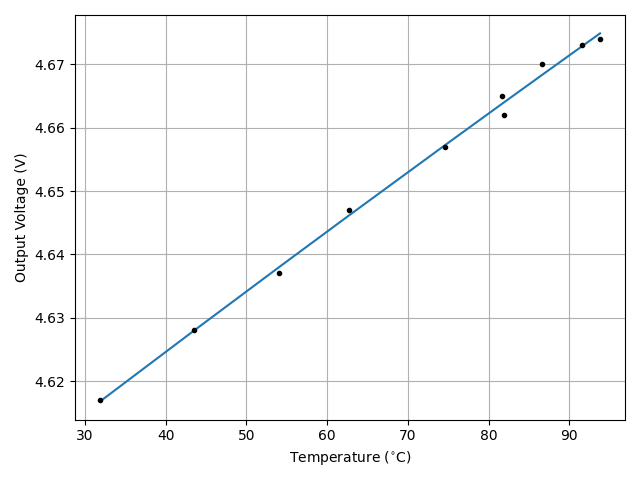
\includegraphics[width=\columnwidth]{figs/train.png}
    \caption{Training the model.}
    \label{fig:train}
\end{figure}

\section{Validation}
The validation dataset is shown in Table \ref{tab:valid}. The results of the 
validation are shown in Fig. \ref{fig:valid}.
\begin{table}[!ht]
    \centering
    \input{tables/validation_data.tex}
    \caption{Validation data.}
    \label{tab:valid}
\end{table}
\begin{figure}[!ht]
    \centering
    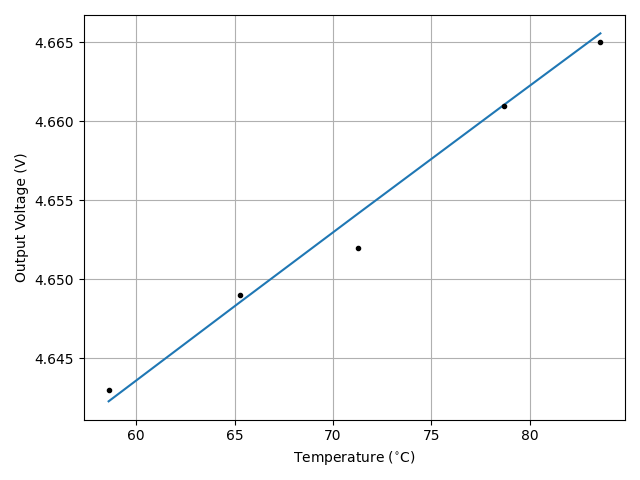
\includegraphics[width=\columnwidth]{figs/valid.png}
    \caption{Validating the model.}
    \label{fig:valid}
\end{figure}

\section{Conclusion}

This lab experiment demonstrates how machine learning methods can be used to 
model the behaviour of an unknown device, and find the right parameters that 
fit the model. It also shows how to use Python libraries and frameworks to
collect data and perform optimization.
\end{document}e